% Copyright (C) 2012 Shi.Zhan <g.shizhan.g@gmail.com>
%
% Permission is hereby granted, free of charge, to any person obtaining a copy of this software and associated documentation files (the "Software"), to deal in the Software without restriction, including without limitation the rights to use, copy, modify, merge, publish, distribute, sublicense, and/or sell copies of the Software, and to permit persons to whom the Software is furnished to do so, subject to the following conditions:
%
% The above copyright notice and this permission notice shall be included in all copies or substantial portions of the Software.
%
% THE SOFTWARE IS PROVIDED "AS IS", WITHOUT WARRANTY OF ANY KIND, EXPRESS OR IMPLIED, INCLUDING BUT NOT LIMITED TO THE WARRANTIES OF MERCHANTABILITY, FITNESS FOR A PARTICULAR PURPOSE AND NONINFRINGEMENT. IN NO EVENT SHALL THE AUTHORS OR COPYRIGHT HOLDERS BE LIABLE FOR ANY CLAIM, DAMAGES OR OTHER LIABILITY, WHETHER IN AN ACTION OF CONTRACT, TORT OR OTHERWISE, ARISING FROM, OUT OF OR IN CONNECTION WITH THE SOFTWARE OR THE USE OR OTHER DEALINGS IN THE SOFTWARE.
%
% 课程:人机交互技术及应用
% 班级:传播学1001班
% 课时:40学时,2012年秋季1~10周,每周一、三
% 地点:东九楼D212
% 主页:http://code.google.com/p/hci-course/
% 教师:施展 
% 单位:华中科技大学 武汉光电国家实验室
%
\documentclass{beamer}
\usepackage{fontspec,xunicode,xltxtra,beamerthemesplit}
%\usetheme{Hannover} % White background
\usetheme{Berkeley} % Blue background
\setmainfont[
	BoldFont={WenQuanYi Zen Hei},
	ItalicFont={WenQuanYi Micro Hei}
]{WenQuanYi Micro Hei}
\setsansfont[
	BoldFont={WenQuanYi Zen Hei},
	ItalicFont={WenQuanYi Micro Hei}
]{WenQuanYi Micro Hei}

% 中文环境自动换行
\XeTeXlinebreaklocale "zh"
\XeTeXlinebreakskip = 0pt plus 1pt

% 中文环境修正导航栏
\makeatletter
\def\beamer@linkspace#1{
	\begin{pgfpicture}{0pt}{-1.5pt}{#1}{5.5pt}
		\pgfsetfillopacity{0}
		\pgftext[x=0pt,y=-1.5pt]{.}
		\pgftext[x=#1,y=5.5pt]{.}
	\end{pgfpicture}
}
\makeatother

% diagrams
\usepackage{tikz}
\usetikzlibrary{arrows,shapes}

% full page image
\newcommand{\fullPageImage}[2]{
	{
		\usebackgroundtemplate{\includegraphics[width=\paperwidth, height=\paperheight]{#1}}
		\frame[plain]{#2}
	}
}

\title{人机交互技术}
\author{施展}
\institute{华中科技大学~武汉光电国家实验室}
\date{\today}
\titlegraphic{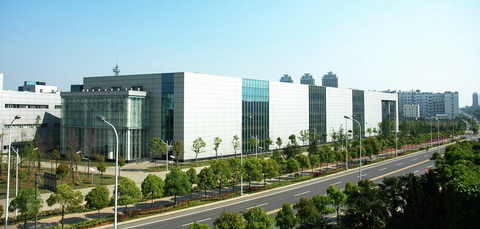
\includegraphics[width=2cm]{images/wnlo.jpg}}

\begin{document}

\begin{frame}
	\titlepage
\end{frame}

\begin{frame}
	\frametitle{内容提要}
	\tableofcontents
\end{frame}

\section{第六讲}
\begin{frame}
	\frametitle{第六讲 人机交互界面表示模型与实现}
	\begin{itemize}
		\item \textbf{目的}: 在界面设计的早期阶段,研究建立一种用户界面表示模型
		\begin{itemize}
			\item 利用形式化的设计语言来分析和表达用户任务以及用户和系统之间的交互情况;
			\item 使界面表示模型能方便地映射到实际的设计实现。
		\end{itemize}
	\end{itemize}
\end{frame}

\subsection{人机交互界面表示模型}
\begin{frame}
	\frametitle{人机交互界面表示模型}
	\beamertemplatetransparentcovereddynamicmedium
	本节介绍人机交互界面主要表示模型及其转换
	\begin{itemize}
		\item 行为模型:\\{\tiny 该模型主要从用户和任务的角度考虑如何来描述人机交互界面。}
		\item 结构模型:\\{\tiny 该模型主要从系统的角度来表示人机交互界面。}
		\item 模型转换:\\{\tiny 主要介绍行为模型到结构模型的转换。}
		\item 表现模型:\\{\tiny 主要介绍人机界面表现的具体描述方法。}
	\end{itemize}
\end{frame}

\begin{frame}
	\frametitle{人机交互界面表示模型~{\small 行为模型}}
	\begin{itemize}
		\item GOMS: Goal, Operator, Method, Selection 
		\item LOTOS: Language Of Temporal Ordering Specification
		\item UAN: User Action Notation
	\end{itemize}
\end{frame}

\begin{frame}
	\frametitle{人机交互界面表示模型~{\small GOMS}}
	\begin{itemize}
		\item 1983年由Card, Morgan和Newell 提出的。
		\item 通过目标 (Goal)、操作 (Operator)、方法 (Method) 以及选择规则 (Selection) 四个元素来描述用户的行为。
		\item GOMS是在交互系统中用来分析、建立用户行为的模型,采用“分而治之”的思想,将一个任务进行多层次的细化。
	\end{itemize}
\end{frame}

\begin{frame}
	\frametitle{人机交互界面表示模型~{\small GOMS}}
	\beamertemplatetransparentcovereddynamicmedium
	\begin{itemize}
		\item 目标 Goals
		\begin{itemize}
			\item 目标就是用户执行任务最终想要得到的结果,它可以在不同的层次中进行定义。
			\item 例: “编辑一篇文章”-“编辑文章”(高层);“删除字符”(低层)
		\end{itemize}
		\pause
		\item 操作 Operators
		\begin{itemize}
			\item 操作是任务分析到最低层时的行为,是用户为了完成任务所必须执行的基本动作。
			\item 操作不能被分解,在GOMS模型中是原子动作。
		\end{itemize}
	\end{itemize}
\end{frame}

\begin{frame}
	\frametitle{人机交互界面表示模型~{\small GOMS}}
	\beamertemplatetransparentcovereddynamicmedium
	\begin{itemize}
		\item 方法 Methods
		\begin{itemize}
			\item 方法是描述如何完成目标的过程。
			\item 一个方法本质上来说是内部的算法,用来确定子目标序列及完成目标所需要的操作。
		\end{itemize}
		\item 选择 Selection
		\begin{itemize}
			\item 选择是用户要遵守的判定规则,以确定在特定环境下所要使用的方法。
			\item 当有多个方法可供选择时,GOMS中并不认为这是一个随机的选择,而是尽量来预测会使用哪个方法,这需要根据特定用户、系统的状态、目标的细节来预测要选择哪种方法。
		\end{itemize}
	\end{itemize}
\end{frame}

\begin{frame}
	\frametitle{人机交互界面表示模型~{\small GOMS}}
	\beamertemplatetransparentcovereddynamicmedium
	\begin{itemize}
		\item 例:窗口最小化
	\end{itemize}
	% http://www.idemployee.id.tue.nl/g.w.m.rauterberg/lecturenotes/id%20lecture-6/sld040.htm
	\begin{center}
	\only<1>{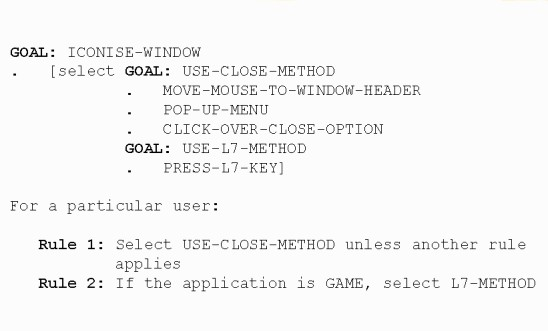
\includegraphics[width=0.7\textwidth]{images/goms-sample-2.jpg}}
	\only<2>{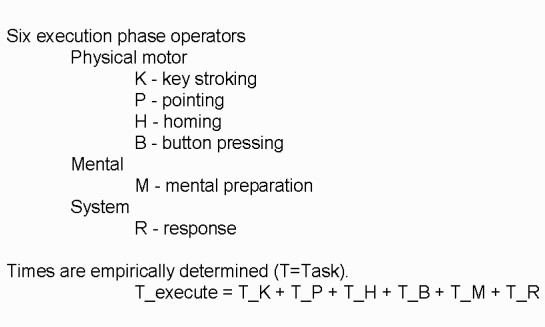
\includegraphics[width=0.7\textwidth]{images/goms-sample-2-1.jpg}}
	\only<3>{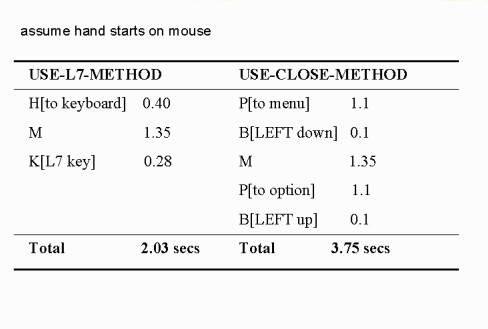
\includegraphics[width=0.7\textwidth]{images/goms-sample-2-2.jpg}}
	\end{center}
\end{frame}

\begin{frame}
	\frametitle{人机交互界面表示模型~{\small GOMS}}
	\beamertemplatetransparentcovereddynamicmedium
	\begin{itemize}
		\item 例:删除文件(命令行)
	\end{itemize}
	\begin{center}
	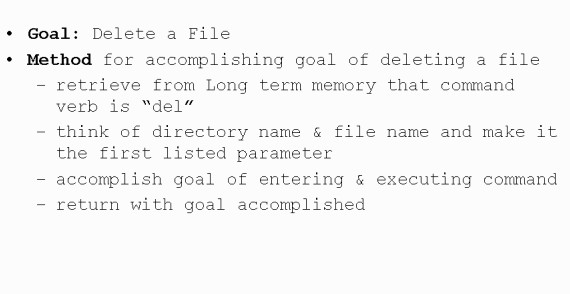
\includegraphics[width=0.7\textwidth]{images/goms-sample-5.jpg}
	\end{center}
\end{frame}

\begin{frame}
	\frametitle{人机交互界面表示模型~{\small GOMS}}
	\beamertemplatetransparentcovereddynamicmedium
	\begin{itemize}
		\item 例:删除文件(图形界面)
	\end{itemize}
	\begin{center}
	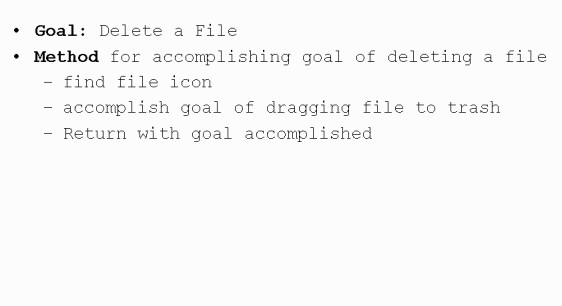
\includegraphics[width=0.7\textwidth]{images/goms-sample-6.jpg}
	\end{center}
\end{frame}

\begin{frame}
	\frametitle{人机交互界面表示模型~{\small GOMS}}
	\beamertemplatetransparentcovereddynamicmedium
	\begin{itemize}[<+->]
		\item 是一种人机交互界面表示的理论模型,被称为最成熟的工程典范~{\tiny 该模型在计算机系统的评估方面也有广泛的应用。}
		\item 没有清楚的描述错误处理的过程,{\tiny 假设用户完全按一种正确的方式进行人机交互,因此只针对那些不犯任何错误的专家用户。}
		\item GOMS对于任务之间的关系描述过于简单,{\tiny 只有顺序和选择,事实上任务之间的关系还有很多种。}
		\item 选择关系通过非形式化的附加规则描述,实现起来比较困难。
		\item 把所有的任务都看作是面向操作目标的,而忽略了一些任务所要解决的问题本质以及用户间的个体差异,{\tiny 它的建立不是基于现有的认知心理学,无法代表真正的认知过程。}
	\end{itemize}
\end{frame}

\begin{frame}
	\frametitle{人机交互界面表示模型~{\small LOTOS}}
	\beamertemplatetransparentcovereddynamicmedium
	\begin{itemize}[<+->]
		\item Language Of Temporal Ordering Specification~\cite{bolognesi1987introduction}
		\item 国际标准形式描述语言,无二义性,适于描述具有并发、交互、反馈和不确定性等特点的并发(concurrent)系统中的行为。
		\item 开始作为一种描述网络协议的语言,由于交互系统、特别是多通道交互系统有并发系统的特点,因此成为用来描述交互系统的行为模型。
	\end{itemize}
\end{frame}

\begin{frame}
	\frametitle{人机交互界面表示模型~{\small LOTOS}}
	\beamertemplatetransparentcovereddynamicmedium
	\begin{itemize}[<+->]
		\item 系统的外部可见行为可以看作是由一个有时序关系的交互序列组成。
		\item 系统由一系列进程组成,进程同环境之间通过称为“关口”(gates)的交互点进行交互。
		\item 两个以上的进程在执行同一个外部可见的行为时会发生交互操作,进行数据交换、信息传递、协调同步等操作。
		\item 进程行为用“行为表达式”来描述,复杂的行为由简单的行为表达式通过表示时序关系的LOTOS算符组合而成。
		\item 在将LOTOS思想用于人机交互的行为模型时,用进程之间的约束关系来描述交互子任务之间的关系。 
	\end{itemize}
\end{frame}

\begin{frame}
	\frametitle{人机交互界面表示模型~{\small LOTOS}}
	\begin{itemize}
		\item LOTOS算符
	\end{itemize}
	\begin{center}
	\begin{tabular}{|c|c|}
	\hline $ T1 \mid\mid\mid T2 $ & 交替 Interleaving \\ 
	\hline $ T1 [] T2 $ & 选择 Choice \\ 
	\hline $ T1 \mid [a_1,\dots,a_n] \mid T2 $ & 同步 Synchronization \\ 
	\hline $ T1 [> T2 $ & 禁止 Deactivation \\ 
	\hline $ T1 \gg T2 $ & 允许 Enabling \\ 
	\hline 
	\end{tabular} 
	\end{center}
\end{frame}

\begin{frame}
	\frametitle{人机交互界面表示模型~{\small LOTOS}}
	\begin{itemize}
		\item 例:中国象棋
	\end{itemize}
	\begin{center}
	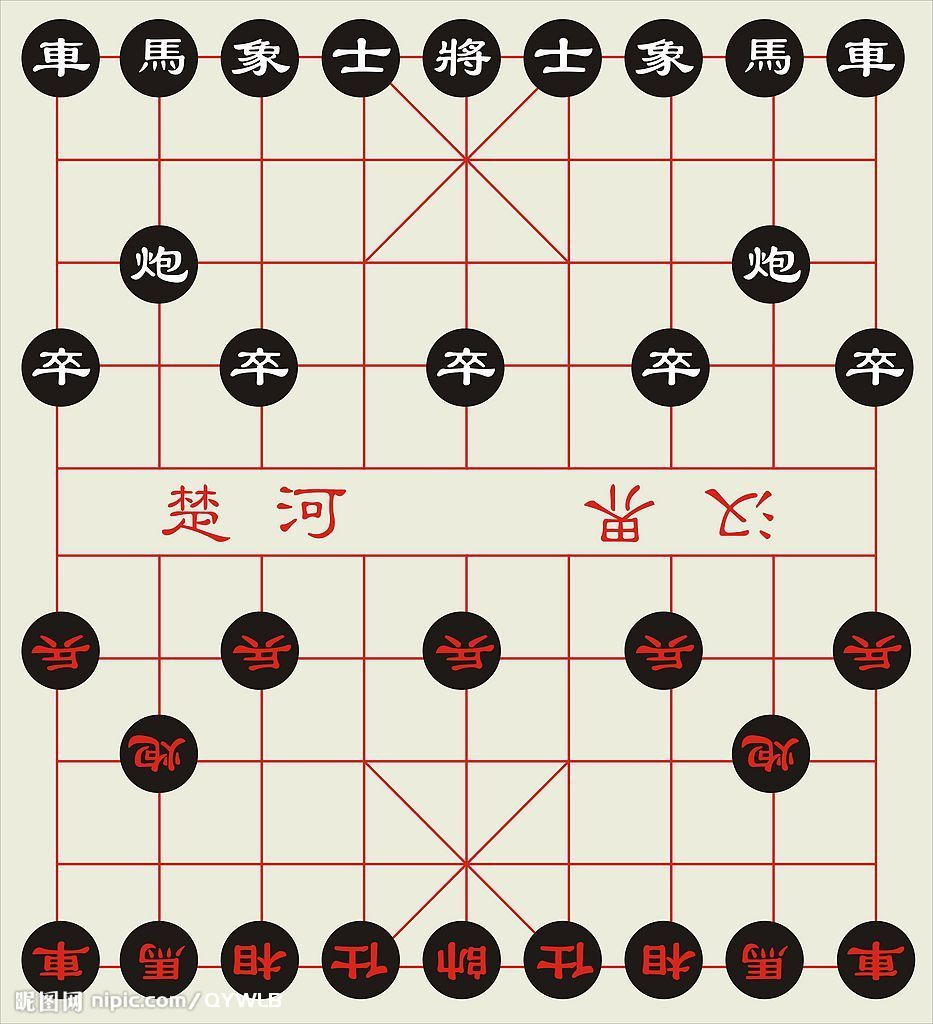
\includegraphics[width=0.5\textwidth]{images/chinese-chess.jpg}
	\end{center}
\end{frame}

\begin{frame}
	\frametitle{人机交互界面表示模型~{\small LOTOS}}
	\begin{center}
	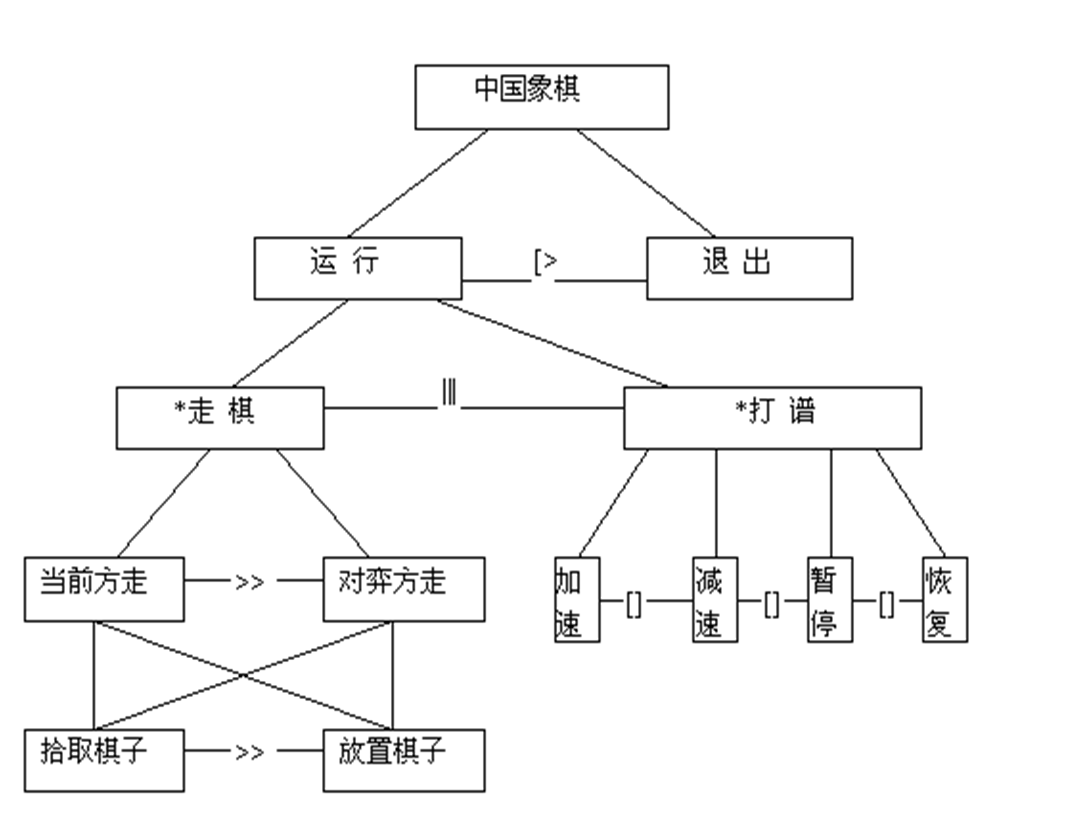
\includegraphics[width=0.7\textwidth]{images/chinese-chess-lotos.png}\\
	{\tiny 中国象棋的LOTOS任务分解实例}
	\end{center}
\end{frame}

\begin{frame}
	\frametitle{LOTOS与GOMS的结合}
	\beamertemplatetransparentcovereddynamicmedium
	\begin{itemize}[<+->]
		\item LOTOS模型很好的描述了任务之间的时序约束关系,这些时序约束关系能更好的描述GOMS中子目标之间的关系。
		\item 用GOMS模型描述任务的分解过程,而用LOTOS给出子任务之间的约束关系,这样就可以增加两种表示模型的表示能力。 
	\end{itemize}
\end{frame}

\begin{frame}
	\frametitle{LOTOS与GOMS的结合}
	\begin{columns}
	\column{.5\textwidth}
	GOAL:中国象棋\\
	~~[>:\\
	~~GOAL:运行\\
	~~~~|||:\\
	~~~~*GOAL:走棋\\
	~~~~~~ACTION:自动记录棋谱\\
	~~~~~~~>>:\\
	~~~~~~GOAL:当前方走\\
	~~~~~~~>>:\\
	~~~~~~~OPRATOR:拾取棋子\\
	~~~~~~~OPRATOR:放置棋子\\
	~~~~~~GOAL:对弈方走\\
	\column{.5\textwidth}
	~~~~~~~>>\\
	~~~~~~~OPRATOR:拾取棋子\\
	~~~~~~~OPRATOR:放置棋子\\
	~~~~*GOAL:打谱\\
	~~~~~~~[]:\\
	~~~~~~~OPRATOR:加速\\
	~~~~~~~OPRATOR:减速\\
	~~~~~~~OPRATOR:暂停\\
	~~~~~~~OPRATOR:恢复\\
	~~GOAL:退出\\
	\end{columns}
\end{frame}

\begin{frame}
	\frametitle{LOTOS与GOMS的结合}
	\beamertemplatetransparentcovereddynamicmedium
	\begin{itemize}[<+->]
		\item LOTOS与GOMS结合,可以清楚地了解整个目标层次及各目标之间的约束关系。但与GOMS同样存在无法描述目标异常结束的缺陷,同时当任务进行选择时用什么规则进行选择并未涉及。
		\item LOTOS最大的优越性在于可以构造一套现成的自动化工具,利用这些工具,可自动进行错误检测,但它过于形式化的记法比较晦涩难懂。
		\item GOMS和LOTOS的结合可以很好地描述人机交互的较高级的任务,对于原子任务的形式化描述,上述模型并没有给出一个比较清晰的描述。
		\item UAN模型主要用于原子目标的描述。
	\end{itemize}
\end{frame}

\begin{frame}
	\frametitle{人机交互界面表示模型~{\small UAN}}
	\beamertemplatetransparentcovereddynamicmedium
	\begin{itemize}[<+->]
		\item User Action Notation~\cite{hartson1990uan}
		\item UAN是一种简单的符号语言,主要描述用户的行为序列以及在执行任务时所用的界面物理对象。 
		\item 尽管UAN属于一种行为模型,但作为一种任务描述语言,它又涉及一定程度的系统行为的描述,因而它兼有行为模型和结构模型的一些特点。
		\item \dots
	\end{itemize}
\end{frame}

\begin{frame}
	\frametitle{人机交互界面表示模型~{\small 结构模型}}
	\begin{itemize}
		\item 产生式规则 Production Rule
		\begin{itemize}
			\item 上下文无关文法,将人机交互对话看作是一种语言,运用基于语法的方法来描述交互对话。
			\item 产生式集合定义了用户与计算机交互所运用的语言。
		\end{itemize}
		\item 状态转换网络 State Transition Network
		\begin{itemize}
			\item 定义一个具有一定数量状态的转换机,称之为有限状态机-Finite State Machine(FSM)。
			\item FSM从外部世界中接收到事件,并能使FSM从一个状态转换到另一个状态。
			\item 两种最基本的状态转换网络,状态转换网络(State Diagrams)和扩展状态转换网络(State Charts),后者是前者的一个扩展。
		\end{itemize}
	\end{itemize}
\end{frame}

\begin{frame}
	\frametitle{人机交互界面表示模型~{\small 行为模型和结构模型的转换}}
	\begin{itemize}
		\item 整体框架
		\item 转换算法
	\end{itemize}
\end{frame}

\begin{frame}
	\frametitle{人机交互界面表示模型~{\small 表现模型}}
	\begin{itemize}
		\item 逻辑组织结构
		\item 面板内部时间分发及响应方式
		\item 面板间关系
	\end{itemize}
\end{frame}

\begin{frame}
	\frametitle{人机交互界面表示模型~{\small 表现模型}}
	\beamertemplatetransparentcovereddynamicmedium
	\begin{itemize}
		\item 表现模型(PM)描述了用户界面的表现形式,由层次性的交互对象组成。
		\begin{itemize}
			\item 交互对象一般由抽象交互对象(AIO - Abstract Interactive Object)和具体交互对象(CIO - Concrete Interactive Object)组成。
		\end{itemize}
		\pause
		\item 管理信息系统的交互界面:填表界面
		\begin{itemize}
			\item 界面元素:界面元素属性,对几何对象、内容对象、绘制对象的描述
			\item 面板:界面元素的模型定义+界面元素的列表和布局的定义
			\item XML描述
		\end{itemize}
	\end{itemize}
\end{frame}

\begin{frame}
	\frametitle{人机交互界面表示模型~{\small 表现模型}}
	\beamertemplatetransparentcovereddynamicmedium
	\begin{itemize}[<+->]
		\item 体验~{\tiny WinSpy}
		\item 数据结构
		\item 属性及响应
	\end{itemize}
\end{frame}

\begin{frame}
	\frametitle{人机交互界面表示模型~{\small 表现模型}}
	\beamertemplatetransparentcovereddynamicmedium
	\begin{itemize}[<+->]
		\item 面板间的关系
		\begin{itemize}
			\item 并列关系
			\item 嵌套关系
			\item 依赖关系~{\tiny 依赖面板、依赖事件}
		\end{itemize}
		\pause
		\item 面板界面分类
		\begin{itemize}
			\item 自由面板 (FreePanel)
			\item 面板面板 (PanelPanel)
			\item 原子面板 (ComponentPanel)
		\end{itemize}
		\pause
		\item 体验~{\tiny QT Designer + XML Spy}
	\end{itemize}
\end{frame}

\subsection{界面描述语言}
\begin{frame}
	\frametitle{界面描述语言}
	\beamertemplatetransparentcovereddynamicmedium
	\begin{itemize}
		\item 命令式语言
		\begin{itemize}
			\item 由编程人员明确指定如何执行任务
			\item C++, Java, Python, 各类过程性语言 \dots
		\end{itemize}
		\pause
		\item 陈述式语言
		\begin{itemize}
			\item 由编程人员说明任务内容和目的
			\item XML, RDF, LaTeX, 各类标记语言 \dots
		\end{itemize}
		\pause
		\item 陈述式语言更为抽象、通用、适合于界面描述。
	\end{itemize}
\end{frame}

\begin{frame}
	\frametitle{常见陈述性界面描述语言}
	\beamertemplatetransparentcovereddynamicmedium
	\begin{itemize}
		\item 用户界面标记语言 UIML
		\begin{itemize}
			\item User Interface Markup Language
			\item 由结构 (structure)、样式 (style)、内容 (content)、行为 (behavior)四个方面来描述~\cite{abrams1999uiml}
			\item 由 Organization for the Advancement of Structured Information Standards (OASIS) 标准化
		\end{itemize}
		\pause
		\item 扩展界面标记语言 XIML
		\begin{itemize}
			\item 由组件 (Components)、关系 (Relations)和属性 (Attributes)三部分构成
			\item 组件:定义了任务、域、用户、表现和对话五类
		\end{itemize}
		\pause
		\item XML用户界面语言 XUL
		\begin{itemize}
			\item 提供创建现代图形界面大多数元素的能力。
		\end{itemize}
	\end{itemize}
\end{frame}

\begin{frame}
	\frametitle{HTML/CSS}
	\beamertemplatetransparentcovereddynamicmedium
	\begin{itemize}
		\item HTML 超文本标签语言
	    \item XHTML 更严谨HTML版本
	    \item HTML 5 下一代的HTML
	    \item CSS 层叠样式表 Cascading Style Sheets
	    \pause
	    \item 体验~{\tiny Chrome}
	\end{itemize}
\end{frame}

\begin{frame}
	\frametitle{XUL}
	\beamertemplatetransparentcovereddynamicmedium
	\begin{columns}
	\column{.5\textwidth}
	\begin{itemize}
		\item XML User Interface Language
		\begin{itemize}
			\item 支持Mozilla系列的应用程序{\tiny (如Mozilla Firefox和Mozilla Thunderbird)}而开发的用户界面标记语言。
			\item 重用了许多现有的标准和技术~{\tiny 包括CSS、JavaScript、DTD和RDF等。}
			\item 主要好处在于提供了一套简易和跨平台的widget定义。
		\end{itemize}
		\pause
		\item 体验~{\tiny QT Designer}
	\end{itemize}
	\column{.5\textwidth}
	% http://starkravingfinkle.org/blog/xul-explorer/
	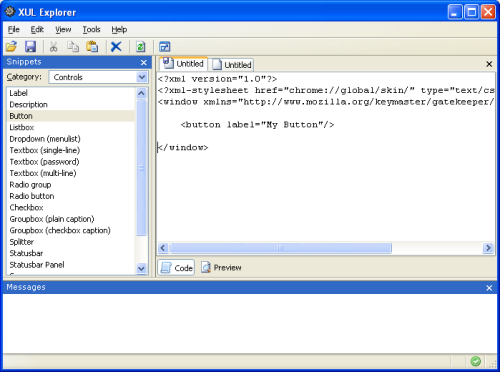
\includegraphics[width=\textwidth]{images/xulexplorer.png}
	\end{columns}
\end{frame}

\subsection{窗口系统}
\begin{frame}
	\frametitle{窗口系统}
	\beamertemplatetransparentcovereddynamicmedium
	\begin{itemize}[<+->]
		\item 对交互应用系统实现三个层次上的支持
		\begin{itemize}
			\item 窗口系统对交互应用系统实现的支持
			\item 软件开发环境对交互应用系统实现的支持
			\item 用户界面管理系统UIMS
		\end{itemize}
	\end{itemize}
\end{frame}

\begin{frame}
	\frametitle{窗口系统结构}
	\beamertemplatetransparentcovereddynamicmedium
	\begin{itemize}
		\item 三种不同结构
		\begin{itemize}
			\item 在各个应用程序内部实现和管理多任务
			\begin{itemize}
				\item 移植起来不方便
				\item 应用程序处理复杂
			\end{itemize}
			\pause
			\item 在操作系统核心集中处理多任务管理
			\begin{itemize}
				\item 过分的依赖操作系统
				\item 移植起来不方便
			\end{itemize}
			\pause
			\item 多任务的管理可由独立的管理程序进行管理
			\begin{itemize}
				\item 应用程序通过调用该管理程序提供的接口来实现对多任务的管理和设备的独立性操作
				\item 最容易移植的
			\end{itemize}
		\end{itemize}
	\end{itemize}
\end{frame}

\begin{frame}
	\frametitle{独立管理程序的客户/服务器结构}
	\begin{itemize}
	\item 以X Window为例
	\end{itemize}
	\begin{center}
	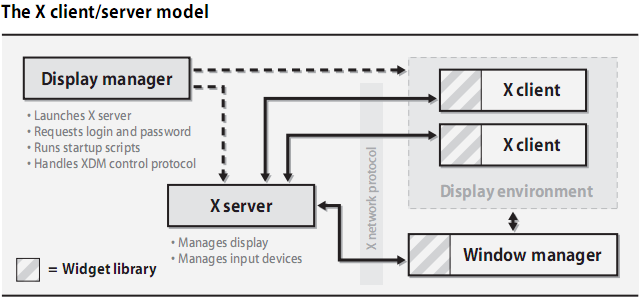
\includegraphics[width=0.9\textwidth]{images/x-server-architecture.png}
	\end{center}
\end{frame}

\begin{frame}
	\frametitle{管理程序组成}
	\beamertemplatetransparentcovereddynamicmedium
	\begin{itemize}
		\item 窗口系统由在服务器端运行的三部分程序组成
		\pause
		\begin{itemize}
			\item 资源管理器
			\begin{itemize}
				\item 整个窗口系统的核心
				\item 负责多任务的管理,并通过设备驱动程序来管理外部设备。
			\end{itemize}
			\pause
			\item 设备驱动程序
			\begin{itemize}
				\item 负责外部设备的驱动,接受输入设备的输入。
				\item 将输入数据转换成统一的格式,通过设备驱动程序实现设备的独立性。
			\end{itemize}
			\pause
			\item 抽象终端
			\begin{itemize}
				\item 负责和客户应用程序的接口
				\item 对每个应用程序由窗口管理程序为其分配一个抽象终端。
			\end{itemize}
		\end{itemize}
	\end{itemize}
\end{frame}

\begin{frame}
	\frametitle{交互事件处理}
	\beamertemplatetransparentcovereddynamicmedium
	\begin{itemize}
		\item 主要有两种形式
		\pause
		\begin{itemize}
			\item 应用程序内部事件处理循环
			\begin{itemize}
				\item 服务器把用户的输入作为事件送给客户应用程序
				\item 客户应用程序对传给它的所有的事件都做出响应,不同的事件采取不同的处理
				\item 早期的基于窗口系统的开发往往采用这种方式
			\end{itemize}
			\pause
			\item 事件注册方式
			\begin{itemize}
				\item 事件处理中心负责事件的处理;
				\item 应用程序登记处理的事件;
				\item 事件处理中心接收事件,把事件和控制转向该事件注册的回应过程;
				\item 处理完后,回应过程把控制返还给事件处理中心。
			\end{itemize}
		\end{itemize}
		\pause
		\item 事件注册方式优点
		\begin{itemize}
			\item 应用程序不需要设计事件处理循环
			\item 事件处理中心处理事件的效率相对比较高
		\end{itemize}
	\end{itemize}
\end{frame}

%\begin{frame}
%	\frametitle{交互组件开发包}
%
%\end{frame}
%
%\begin{frame}
%	\frametitle{交互框架}
%
%\end{frame}
%
%\begin{frame}
%	\frametitle{MVC模型及Structs结构}
%
%\end{frame}

\subsection{用户界面管理系统}
\begin{frame}
	\frametitle{用户界面管理系统}
	\beamertemplatetransparentcovereddynamicmedium
	\begin{itemize}[<+->]
		\item 一个支持交互系统开发的UIMS的概念结构
		\item 该结构把应用程序的语义与表现分开
		\item 保留应用程序和表示形式之间的内在关系
		\item 支持运行的交互系统的管理、实现和评估的技术
	\end{itemize}
\end{frame}

\begin{frame}
	\frametitle{UIMS的表示方法}
	\beamertemplatetransparentcovereddynamicmedium
	\tikzstyle{block} = [
		rectangle,
		rounded corners,
		draw=black, very thick,
		fill=blue!20,
		text width=8em,
		minimum height=2em,
		text centered]
	\tikzstyle{line} = [
		draw, -latex',
		draw=black, very thick,
		text centered]

	\begin{columns}
	\column{.3\textwidth}
	\begin{center}
	\begin{tikzpicture}[node distance=1.3cm, auto,]
		\node[] (a) {用户};
		\uncover<2->{
			\node[block, below of = a] (b) {表现层};
			\path[line]	(a)--(b);
		}
		\uncover<3->{
			\node[block, below of = b] (c) {对话控制};
			\path[line]	(b)--(c);
		}
		\uncover<4->{
			\node[block, below of = c] (d) {应用层};
			\path[line]	(c)--(d);
		}
		\uncover<1->{
			\node[, below of = d] (e) {应用程序};
			\path[line]	(d)--(e);
		}
	\end{tikzpicture}
	\end{center}
	\column{.7\textwidth}
	\begin{itemize}
		\uncover<2->{
			\item 表现层表示方法
			\begin{itemize}
				\item {\tiny 用户输入输出信息、图形表示的处理}
				\item {\tiny 适应多媒体的需要、智能人机界面规格说明}
			\end{itemize}
		}
		\uncover<3->{
			\item 对话控制的表示方法
			\begin{itemize}
				\item 基于语言的表示方法\\
				{\tiny 菜单网络,状态转换网络\dots}
				\item 基于图形的表示方法\\
				{\tiny 用户使用鼠标器直接将对象放到屏幕上来定义界面}
				\item 基于应用语义过程的表示方法
			\end{itemize}
		}
		\uncover<4->{
			\item 应用层的表示方法
			\begin{itemize}
				\item {\tiny 有关应用数据结构、子程序、及对用户的限制}
				\item {\tiny 排除可能引起语义错误的操作}\\{\tiny 避免对应用程序的破坏}
			\end{itemize}
		}
	\end{itemize}
	\end{columns}
\end{frame}

% http://technet.microsoft.com/en-us/library/bb463223.aspx
\fullPageImage{images/x-client-server.jpg}{}
\fullPageImage{images/x-window-architecture.jpg}{}

% http://msdn.microsoft.com/en-us/library/windows/desktop/ff684176%28v=vs.85%29.aspx
\fullPageImage{images/windows-graphics-apis.jpg}{}
% http://blogs.msdn.com/b/directx/archive/2009/09/29/comparing-direct2d-and-gdi.aspx
\fullPageImage{images/evolution-of-gdi-display-rendering.jpg}{}

\begin{frame}
	\frametitle{Windows Presentation Foundation}
	\begin{center}
	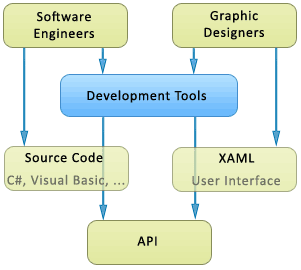
\includegraphics[width=0.5\textwidth]{images/wpf-model.png}
	\end{center}
	其底层使用 Extensible Application Markup Language (XAML)
	% http://sharpertutorials.com/windows-presentation-foundation/
\end{frame}

% http://pic002.cnblogs.com/img/terryfeng/200901/2009012818285931.png
\fullPageImage{images/jquery-api-1.2.png}{}
% http://res.congci.com/upload/image/small/jQuery-Map20091022.png
\fullPageImage{images/jquery-map20091022.png}{}
% http://webdesignerwall.com/tutorials/jquery-tutorials-for-designers
\fullPageImage{images/jquery-how-it-works.jpg}{
	\pause
	\begin{beamerboxesrounded}[shadow=true]{jQuery}
	\begin{itemize}
	\item 是一个 JavaScript 库
	\item 极大地简化了 JavaScript 编程
	\item 很容易学习
	\end{itemize}
	\end{beamerboxesrounded}
}

\section{小结}
\begin{frame}
	\frametitle{小结}
	\begin{itemize}
		\item 理解人机交互界面表示模型
		\item 了解界面描述语言、窗口系统、用户界面管理系统
	\end{itemize}
\end{frame}

\begin{frame}
	\frametitle{参考文献}
	\bibliographystyle{plain}
	\bibliography{hci}
\end{frame}

\end{document}